\documentclass[12pt]{article}

\usepackage[margin=1in]{geometry}
\usepackage[T1]{fontenc}
\usepackage[utf8]{inputenc}
\usepackage{setspace}
\usepackage{graphicx}
\usepackage{float}
\usepackage{booktabs}
\usepackage{tabularx}
\usepackage{longtable}
\usepackage{array}
\usepackage{listings}
\usepackage[table]{xcolor}
\usepackage{hyperref}
\usepackage{enumitem}
\usepackage{caption}
\usepackage{url}
\usepackage{microtype}
\usepackage{titlesec}

\hypersetup{
  colorlinks=true,
  linkcolor=black,
  urlcolor=blue,
  citecolor=black
}

\setstretch{1.18}
\setlength{\parindent}{0pt}
\setlength{\parskip}{0.38em}
\renewcommand{\arraystretch}{1.12}
\setlength{\floatsep}{0.65em}
\setlength{\textfloatsep}{0.75em}
\setlength{\intextsep}{0.65em}
\captionsetup{font=small, labelfont=bf, skip=4pt}
\setlist{topsep=0.25em, itemsep=0.12em, parsep=0pt, partopsep=0pt}
\titlespacing*{\section}{0pt}{1.4ex plus 0.4ex minus 0.2ex}{0.8ex}
\titlespacing*{\subsection}{0pt}{1.0ex plus 0.3ex minus 0.2ex}{0.45ex}
\titlespacing*{\subsubsection}{0pt}{0.8ex plus 0.2ex minus 0.1ex}{0.35ex}
\raggedbottom
\clubpenalty=10000
\widowpenalty=10000
\displaywidowpenalty=10000

\newcolumntype{L}[1]{>{\raggedright\arraybackslash}p{#1}}
\newcolumntype{Y}{>{\raggedright\arraybackslash}X}
\newcommand{\code}[1]{\path{#1}}
\newcommand{\tablegridon}{\arrayrulecolor{black!35}}
\newcommand{\tablegridoff}{\arrayrulecolor{black}}
\newcommand{\tabrowsep}{\\[0.12em]\hline}

\lstset{
  basicstyle=\ttfamily\small,
  frame=single,
  breaklines=true,
  columns=fullflexible,
  keepspaces=true,
  showstringspaces=false
}

\newcommand{\reportfigure}[4][0.95\textwidth]{%
\begin{figure}[H]
\centering
\IfFileExists{#2}{%
  \includegraphics[width=#1]{#2}%
}{%
  \IfFileExists{docs/screenshots/#2}{%
    \includegraphics[width=#1]{docs/screenshots/#2}%
  }{%
    \fbox{\parbox[c][2.75in][c]{0.9\textwidth}{\centering
      Placeholder for figure\\[0.5em]
      Expected file: \code{#2}}}%
  }%
}%
\caption{#3}
\label{#4}
\end{figure}
}

\begin{document}

\begin{titlepage}
\centering

{\LARGE UR3e Web Control\par}
\vspace{0.35in}
{\Large A Senior Project Report\par}

\vspace{0.8in}
presented to\\
the Faculty of California Polytechnic State University\\
San Luis Obispo

\vspace{0.6in}
In Partial Fulfillment\\
of the Requirements for the Degree\\
Bachelor of Science in Computer Engineering

\vspace{0.6in}
By\\
Tenzin Konchok

\vspace{0.8in}
March 2026

\vspace{0.6in}
Advised by Dr.~Javier Gonzalez-Sanchez
\end{titlepage}

\pagenumbering{roman}

\section*{Abstract}
This project investigates how a Universal Robots UR3e can be controlled through a browser-based interface rather than through low-level robot commands alone. The final system supports three interaction modes: chess-style board movement and suction-based pick/place, tic-tac-toe movement and pen-based marking, and whiteboard drawing from uploaded raster images. The implementation combines a React frontend, a Node.js/Express backend, calibrated workspace mapping, URScript generation, RTDE-based live status feedback, and an OpenCV-based drawing pipeline.

The main engineering result is an integrated control platform that translates operator inputs, such as board squares, tic-tac-toe cells, and raster images, into executable robot actions. The system includes dry-run support, single-client control locking, drawing safety checks, and preview support for image-based drawing. The work is best framed as an engineering implementation that connects existing robot interfaces into one usable workflow, not as a new robotics algorithm.

Due to limited project time, development and validation were completed in URSim rather than on the physical robot. The evaluation covers the software workflow, generated URScript path, preview metrics, and simulator-side status behavior, but it does not cover physical placement accuracy, suction reliability, pen contact quality, or real hardware timing. The main limitations are calibration sensitivity, image-quality dependence in whiteboard mode, and ETA estimates that remain approximate rather than exact. Overall, the project provides a structured control platform and a practical foundation for future hardware testing.

\newpage
\pagenumbering{arabic}

\section{Problem Statement}
Universal Robots provides low-level external interfaces such as URScript, RTDE, and dashboard control, but those interfaces do not by themselves provide a complete operator workflow for structured educational and laboratory interaction modes such as board manipulation or image-driven drawing. As a result, there is a gap between raw robot communication and a usable system in which an operator can select a task, preview behavior, and execute it through a single browser-based interface.

The engineering problem addressed in this project is how to build a web control system for a Universal Robots UR3e that can translate user inputs, such as chess squares, tic-tac-toe cells, and uploaded raster images, into calibrated robot actions while maintaining safe execution flow, clear system state, and modular software structure. The system also needs to support multiple task modes within one interface and remain practical for URSim-based development before any physical deployment.

This project addresses that problem by integrating frontend interaction, backend routing, calibration-aware mapping, image vectorization, URScript generation, and live status monitoring into one control platform. The resulting system provides structured task execution rather than only low-level command dispatch.

\section{Goals, Objectives, and Scope}
The formal goal of this project was to develop and validate, in URSim, a web-based control platform for the Universal Robots UR3e that converts user inputs into calibrated robot actions. The system was intended to support board movement, suction-based pick/place, pen-based tic-tac-toe marking, and whiteboard drawing from raster images while maintaining safe execution flow and observable system state. Completion evidence was defined as end-to-end operation of all three modes through a single dashboard, preview and safety support for drawing jobs, and improved moving/idle feedback through RTDE-assisted monitoring.

\subsection{Objectives}
The primary objective of this project was to design and implement a web-based control platform for the Universal Robots UR3e that could support multiple task modes from a single browser interface.

The system was intended to:
\begin{itemize}[leftmargin=*]
\item move the robot to calibrated board positions
\item support chess-style suction pick/place interaction
\item support tic-tac-toe movement and pen-based marking
\item support whiteboard drawing from uploaded PNG/JPG images
\item provide dry-run, control locking, and live status feedback
\item remain usable in URSim as the primary development and validation environment
\end{itemize}

\subsection{Target Success Criteria}
The target success criteria were:
\begin{itemize}[leftmargin=*]
\item board targets could be translated into calibrated poses and executable URScript
\item chess and tic-tac-toe actions could be executed through the web interface without manual backend interaction
\item uploaded raster images could be previewed and executed as drawing plans
\item the system could reject oversized drawing jobs before execution
\item the UI could reflect robot moving/idle state more accurately than fixed timing alone
\item all three modes could operate within one dashboard and one backend architecture
\end{itemize}

\subsection{Included Scope}
The implemented scope includes:
\begin{itemize}[leftmargin=*]
\item a React and TypeScript frontend dashboard
\item a Node.js and Express backend API
\item board calibration and whiteboard calibration profiles
\item URScript generation and TCP dispatch to URSim
\item RTDE-based live motion monitoring with dashboard fallback
\item OpenCV contour extraction, stroke normalization, and planning
\item simulator-based testing in URSim
\end{itemize}

\subsection{Excluded Scope}
The project does not include:
\begin{itemize}[leftmargin=*]
\item full physical robot validation
\item automatic calibration
\item camera-based closed-loop correction
\item robust SVG or text drawing support
\item exact physical runtime prediction for whiteboard ETA
\end{itemize}

\section{Project Overview and Technical Approach}
This project is a web-based control platform for the Universal Robots UR3e focused on structured user interaction rather than low-level robot control alone. It combines frontend interaction, backend routing, calibration-aware mapping, URScript generation, and live robot status feedback into one system. The platform was designed for educational and laboratory workflows in which a user can select a task from a browser interface and have it translated into calibrated robot behavior.

\subsection{Technical Approach}
The technical approach was defined around three intentional layers. First, a web-based control layer in the React frontend and Express backend exposes robot operations through a single dashboard. Second, a calibration-based mapping layer converts board squares, tic-tac-toe cells, and normalized whiteboard coordinates into robot poses using manually defined anchors and local workspace frames. Third, an image-to-trajectory layer converts uploaded raster images into contour strokes, simplified drawing plans, safety-checked motion sequences, and executable URScript. These layers were designed to work together so that multiple task modes could share transport, control locking, status reporting, and calibration concepts instead of being implemented as unrelated demonstrations.

The implemented system supports three operating modes: chess-style board movement and suction-based pick/place, tic-tac-toe movement and pen-based marking, and whiteboard drawing from uploaded raster images. These modes were selected as complementary evaluation cases for the same architecture: target-based movement, grid-based marking, and image-driven trajectory generation. Together, they provide a broader evaluation of the control platform than a single-purpose demo would allow.

The main engineering result is a unified URSim-based platform that integrates multiple interaction modes within one interface and one backend architecture. Because validation was limited to URSim, the current result validates the software architecture, calibration workflow, and execution pipeline in simulation, but it does not establish final hardware performance.

Figure~\ref{fig:multi-mode-interface} shows the final dashboard with the three supported operating modes.

\reportfigure[0.78\textwidth]{new_figures/MultiUI.png}{Multi-mode browser dashboard.}{fig:multi-mode-interface}

\section{Background and Related Work}
The project combines several common ideas from robotics, human-robot interaction, and software systems. At the interaction level, the system follows a supervisory-control pattern: the operator gives structured task commands through a software interface and monitors feedback from the robot instead of manually commanding every low-level motion. This is consistent with established human-robot interaction and telerobotics work, where usability, feedback, and the separation between operator intent and robot execution are central concerns~\cite{goodrich-schultz,hokayem-spong}.

The calibration part of the project uses manually defined anchor points to construct a workspace frame. In this system, anchors define both the board frame for chess and tic-tac-toe interaction and the whiteboard plane for drawing. Once those frames are established, user-level targets can be converted into robot poses. This is simpler than full hand-eye calibration, but it is related to the broader calibration problem in robotics, where coordinate frames must be mapped reliably before robot motion can be trusted~\cite{tsai-lenz,calibration-review}.

The second major idea is task-to-command translation. Instead of issuing robot commands directly at the UI layer, the backend converts targets into URScript and sends them over TCP to URSim. The whiteboard mode adds an image-processing stage, where raster images are converted into contour strokes with OpenCV, normalized into the drawing frame, simplified, and then translated into robot motion. This is related to robotic sketching systems that combine image processing, path planning, and automatically generated robot control code~\cite{robotic-sketching}. In this project, the same architecture supports three task modes rather than a single-purpose drawing workflow.

This project builds directly on the official Universal Robots external interfaces, especially URScript for motion commands, RTDE for telemetry, and the dashboard server for fallback controller status.

\section{Requirements and Evaluation Criteria}
\subsection{Functional Requirements}
\begin{itemize}[leftmargin=*]
\item Move the robot to selected board or drawing targets.
\item Toggle suction for pick/place experiments.
\item Draw X and O marks in tic-tac-toe mode.
\item Accept raster image input and generate drawable strokes.
\item Provide preview, execute, and stop actions for whiteboard drawing.
\item Expose control and status through REST endpoints.
\end{itemize}

\subsection{User Interaction Requirements}
\begin{itemize}[leftmargin=*]
\item Select operating mode and target from a single dashboard.
\item Upload an image, tune parameters, preview, and execute.
\item View connection state, robot state, command feedback, and ETA.
\item Switch calibration profiles from the UI.
\end{itemize}

\subsection{Non-Functional Requirements}
\begin{itemize}[leftmargin=*]
\item Safety: reject oversized drawing jobs before execution.
\item Reliability: UI status should track motion as closely as possible.
\item Performance: commands should dispatch quickly in simulator use.
\item Maintainability: logic should stay modular across routes and robot interfaces.
\item Portability: the system should work in URSim first, with a path toward hardware later.
\end{itemize}

\subsection{Evaluation Criteria}
\begin{itemize}[leftmargin=*]
\item Accuracy: board targets should resolve to the intended region after calibration.
\item Repeatability: repeated tasks should behave consistently in URSim.
\item Status fidelity: moving/idle UI state should match observed robot behavior.
\item Safety compliance: oversized jobs should be blocked with clear feedback.
\item Usability: the main workflows should run without manual backend calls.
\end{itemize}

\subsection{Requirements To Evaluation Traceability}
Table~\ref{tab:traceability} connects the main requirements to the design choices that address them, the modules that implement them, and the evidence collected during evaluation.

\begin{table}[H]
\centering
\caption{Traceability from requirements to evaluation.}
\label{tab:traceability}
\small
\tablegridon
\begin{tabularx}{\textwidth}{|L{2.8cm}|L{3.7cm}|L{4.0cm}|Y|}
\toprule
Requirement & Design Response & Implementation Modules & Evaluation Evidence and Limit \\
\midrule
Board movement and marking & map UI targets through calibrated board frame & \code{move.js}, \code{squares.js} & URSim paths verified; hardware placement and pen contact not measured \tabrowsep
Chess pick/place & share board calibration; separate pick/place actions & \code{move.js}, \code{urTcp.js}, board UI & UI flow and URScript sequencing verified; suction transfer remains hardware work \tabrowsep
Whiteboard drawing & vectorize image, plan strokes, check safety, generate URScript & \code{draw.js}, \code{vectorizeImage.js}, \code{planner.js}, \code{whiteboard.js} & preview metrics measured for three images; physical drawing quality not measured \tabrowsep
Safe execution & support preview, dry run, control lock, and job limits & \code{control.js}, \code{draw.js}, \code{App.tsx} & oversized-job checks and lock behavior exercised in URSim \tabrowsep
Live status feedback & RTDE primary; dashboard fallback & \code{urRtde.js}, \code{urDashboard.js}, \code{state.js} & UI state followed simulator motion; exact latency not quantified \tabrowsep
Dashboard usability & combine modes, target input, preview, execution, and status & \code{App.tsx}, \code{AppHeader.tsx}, \code{WorkspaceBoard.tsx} & all workflows exercised from browser; no formal user study \\
\bottomrule
\end{tabularx}
\tablegridoff
\end{table}

\section{System Design}
The system is organized as a layered web-to-robot architecture with five main component groups: the frontend dashboard, backend route handlers, calibration modules, the drawing pipeline, and robot interface modules. In repository terms, these responsibilities are primarily organized under \code{UI/src}, \code{backend/src/routes}, \code{backend/src/robot}, and \code{backend/src/draw}. The frontend collects user input and displays status, the route handlers validate requests and coordinate task execution, the calibration modules convert workspace coordinates into poses, the drawing pipeline converts raster inputs into normalized strokes, and the robot interface modules handle URScript transport and live state monitoring.

\subsection{Architecture Style}
The overall architecture is best described as a layered, pipeline-based architecture. The layered part separates user interaction, request handling, task planning, and robot communication. The React frontend is responsible for operator input and feedback, the Express route layer validates requests and coordinates workflows, the calibration and drawing modules transform user targets into robot-ready geometry, and the robot interface modules handle URScript, RTDE, and dashboard communication.

The pipeline part appears in how each task moves through the system. A board command follows a short pipeline from selected square or cell, to calibrated pose, to generated URScript, to URSim or UR3e execution. The whiteboard workflow extends that pipeline with image vectorization, stroke simplification, safety checks, and preview metrics before command generation. This architecture was chosen because it keeps each transformation explicit and replaceable. For example, a future hardware test can improve calibration or timing measurement without changing the frontend, and a future drawing workflow can replace the OpenCV vectorizer without rewriting the robot communication layer. Similar web-based robotic systems also emphasize modular architecture and browser-based accessibility for maintainability and portability~\cite{web-telepresence}.

\subsection{Software Design Blueprint}
Figure~\ref{fig:system-pipeline} summarizes the implemented architecture as modules and data flows. The diagram shows the browser interface, backend API, calibration layer, drawing/vectorization pipeline, URScript transport, URSim/UR3e execution, and live status feedback path. Table~\ref{tab:components} then expands that diagram into the specific frontend components, backend route controllers, calibration modules, drawing modules, and robot communication modules used in the implementation.

For chess and tic-tac-toe, the backend maps user-selected targets into calibrated poses and generates URScript directly. For whiteboard drawing, the backend first converts an uploaded raster image into contour strokes, simplifies them, checks safety limits, and only then generates robot motion. This design keeps image processing, geometry, and command transport separated instead of mixing them into a single control file.

\vspace{5.0 em}

\reportfigure[0.99\textwidth]{new_figures/System_Pipeline.png}{Software blueprint and command/status flow.}{fig:system-pipeline}

\subsection{Deployment View}
Figure~\ref{fig:deployment-diagram} complements the software pipeline by showing how the system is deployed at runtime. The browser UI communicates with the Node.js/Express backend through REST requests and status polling. The backend calls the Python/OpenCV vectorization pipeline as a local subprocess for image-based drawing, generates URScript for robot motion, and communicates with URSim or the UR3e controller through URScript TCP, RTDE, and dashboard interfaces.

\vspace{1.0 em}

\reportfigure[0.99\textwidth]{new_figures/Deployment_Diagram.png}{Runtime deployment view.}{fig:deployment-diagram}

\subsection{Module-Level Design}
Figure~\ref{fig:module-system} presents the same implementation from a software design perspective. Instead of showing runtime deployment, it shows the major source modules, their responsibilities, selected functions, and the dependencies between the frontend, route controllers, calibration modules, drawing pipeline, robot communication modules, and status feedback path.

\begin{figure}[H]
\centering
\hspace*{0.18in}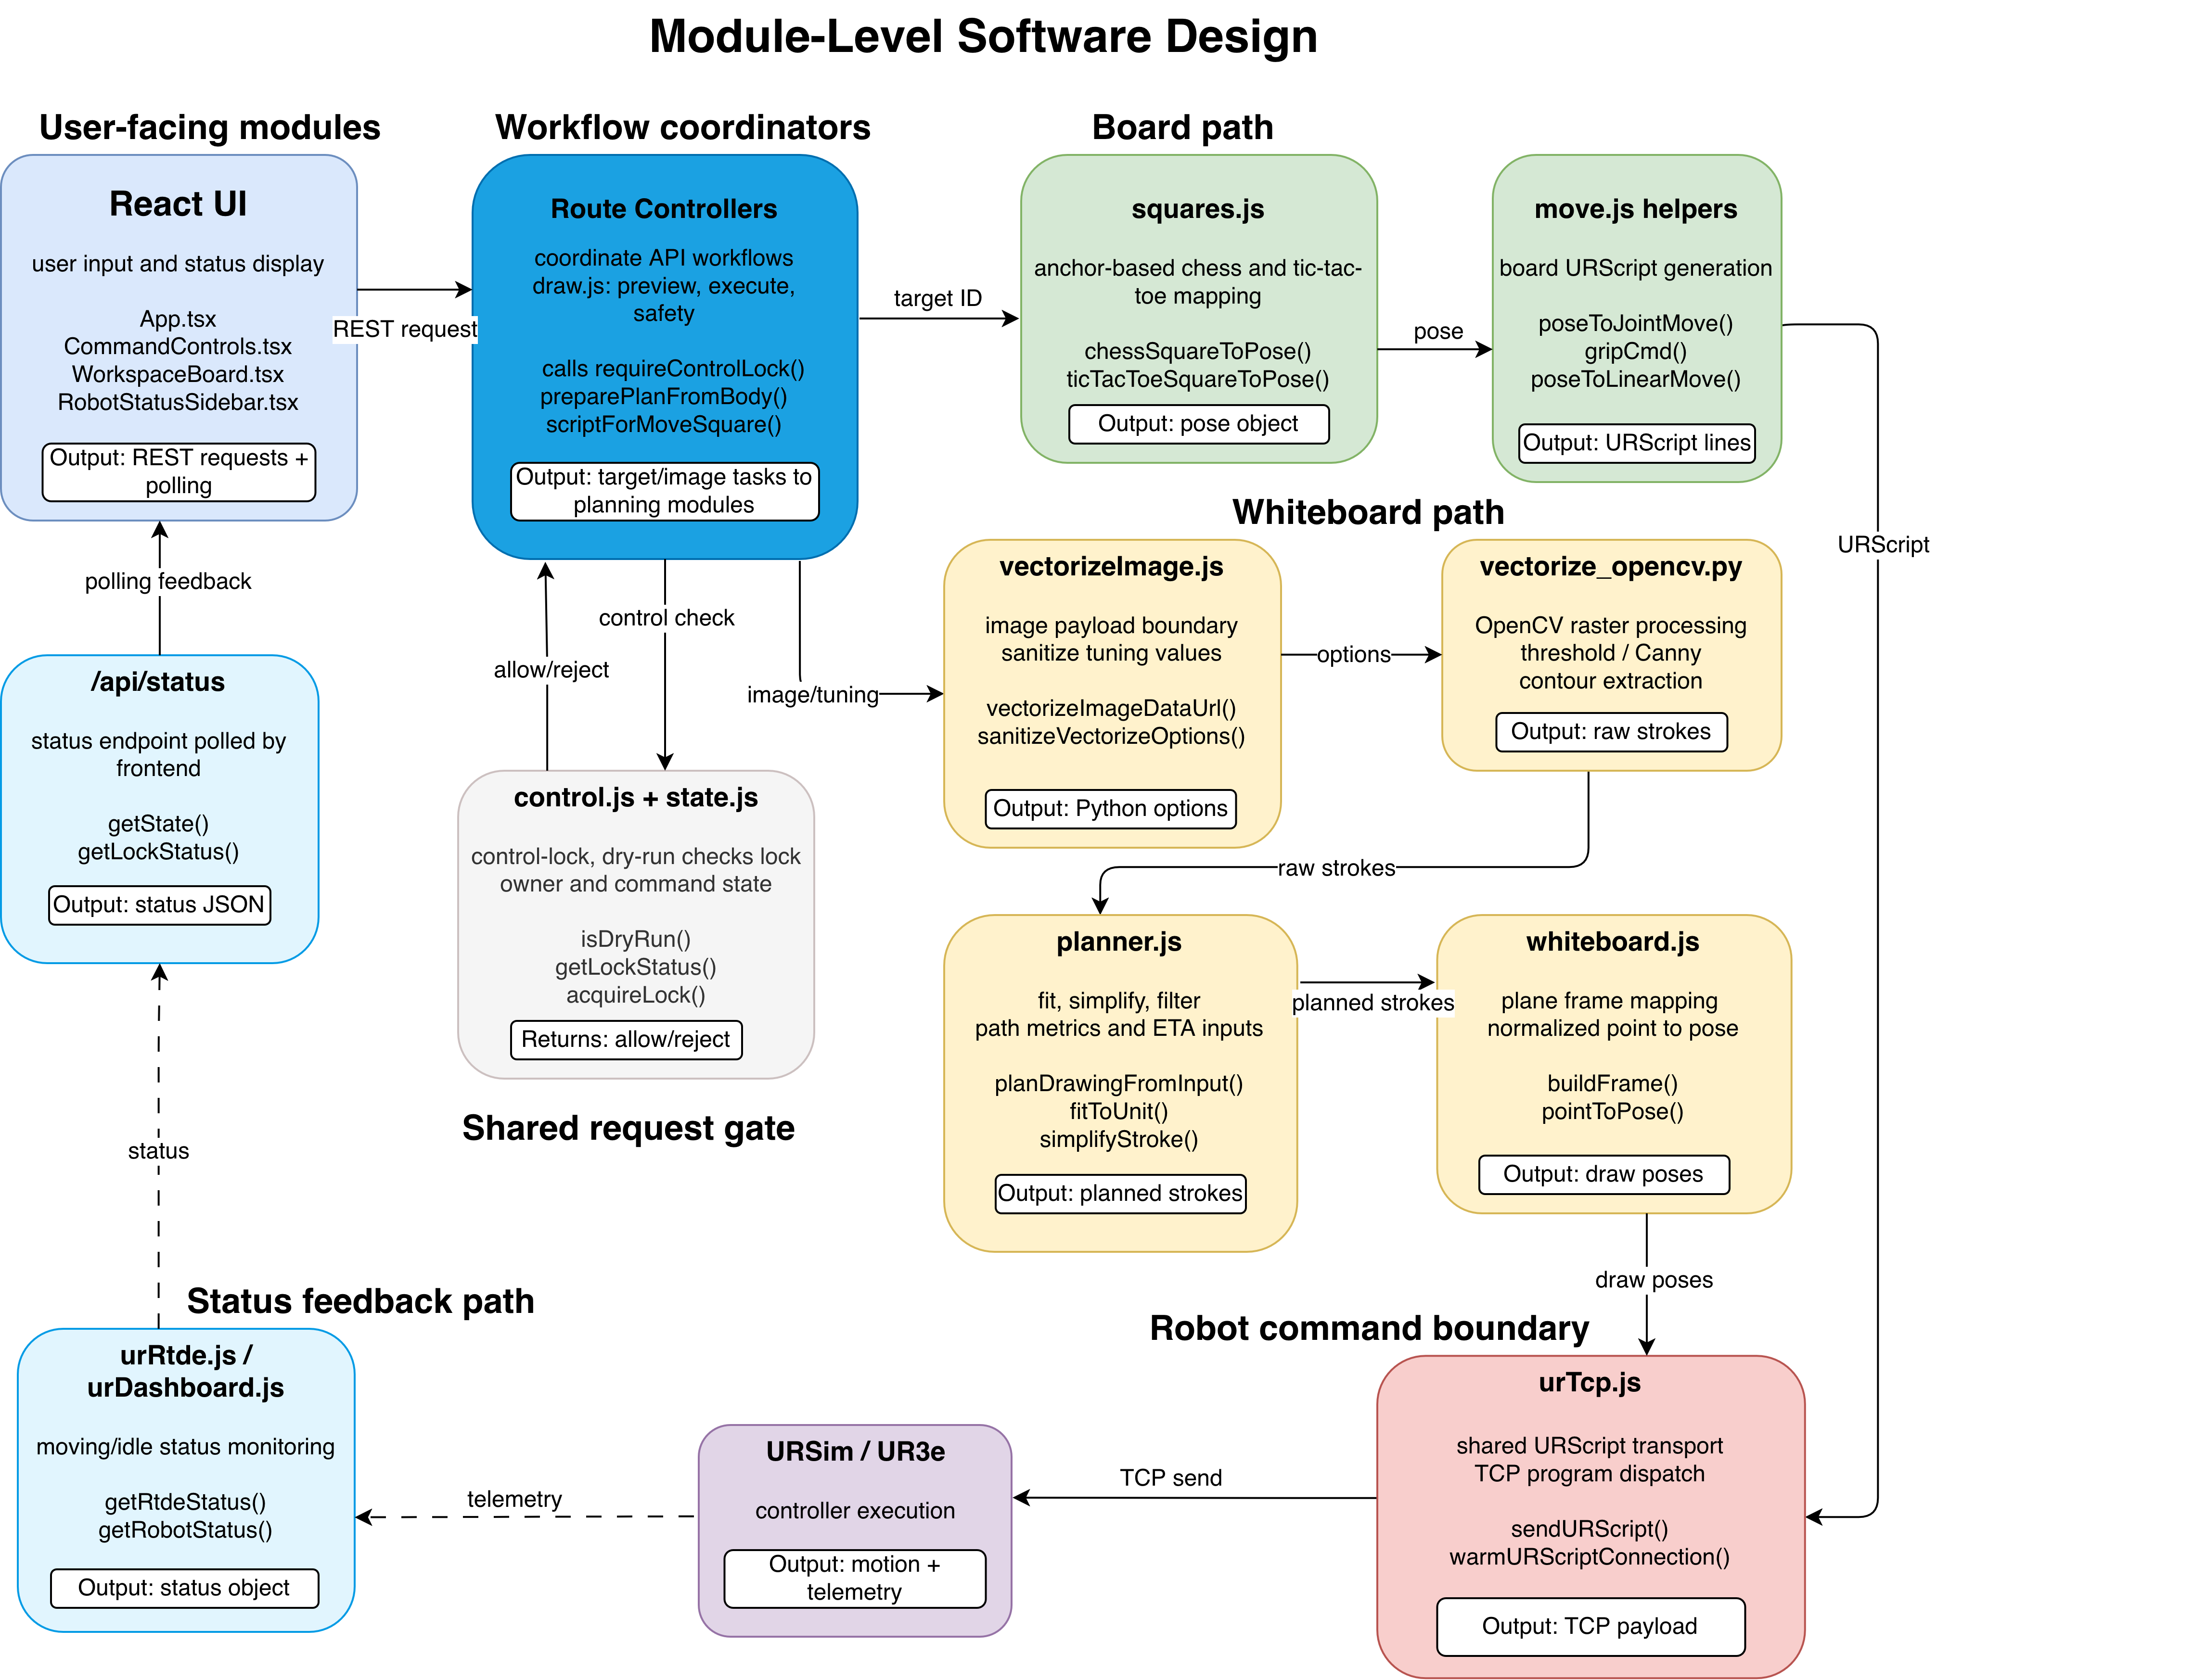
\includegraphics[width=1.17\textwidth]{docs/screenshots/Module_System.png}
\caption{Module-level software design showing major modules, selected functions, outputs, and dependencies.}
\label{fig:module-system}
\end{figure}

\clearpage
\subsection{Module Responsibilities}
\begingroup
\setlength{\tabcolsep}{4pt}
\small
\tablegridon
\begin{longtable}{|L{3.0cm}|L{4.0cm}|L{4.0cm}|L{4.0cm}|}
\caption{Software blueprint module responsibilities.}
\label{tab:components}\\
\toprule
Component & File / Module & Responsibility & Interaction / Data Flow \\
\midrule
Frontend shell & \code{UI/src/App.tsx}, \code{AppHeader.tsx} & mode selection, lock ownership, API coordination & sends REST requests and stores UI state \tabrowsep
Workspace display & \code{WorkspaceBoard.tsx} & board/grid rendering and drawing preview & visualizes selected targets and strokes \tabrowsep
Command controls & \code{CommandControls.tsx} & movement, upload, tuning, preview, execute, stop & builds request payloads \tabrowsep
Status sidebar & \code{RobotStatusSidebar.tsx} & connection, moving/idle, lock owner, drawing metrics & displays backend status payloads \tabrowsep
Movement API & \code{backend/src/routes/move.js} & chess and tic-tac-toe actions & maps square/cell requests to URScript \tabrowsep
Draw API & \code{backend/src/routes/draw.js} & whiteboard preview, execute, stop, ETA, safety & coordinates vectorization, planning, and script generation \tabrowsep
Control gate & \code{backend/src/routes/control.js} & dry-run and single-client ownership & approves or rejects requests \tabrowsep
Board calibration & \code{backend/src/robot/squares.js} & board frame from anchors & maps target ids to board poses \tabrowsep
Whiteboard calibration & \code{backend/src/robot/whiteboard.js} & whiteboard plane mapping & maps normalized strokes to draw poses \tabrowsep
OpenCV vectorizer & \code{backend/src/draw/vectorize\_opencv.py} & contour extraction & converts image input into contour strokes \tabrowsep
Planner & \code{backend/src/draw/planner.js} & fit, simplify, measure strokes & returns strokes, points, path length, and ETA inputs \tabrowsep
URScript transport & \code{backend/src/robot/urTcp.js} & command dispatch & sends URScript over TCP \tabrowsep
RTDE monitor & \code{backend/src/robot/urRtde.js} & moving/idle inference & converts telemetry into UI status \tabrowsep
Dashboard fallback & \code{backend/src/robot/urDashboard.js} & controller fallback status & supplies connection and running state \\
\bottomrule
\end{longtable}
\tablegridoff
\endgroup

The code organization mirrors these component boundaries. Shared request and control-lock behavior is centralized in \code{backend/src/routes/control.js}, board-task logic remains in \code{move.js}, drawing-specific logic remains in \code{draw.js} and \code{backend/src/draw}, and transport / status logic remains isolated in \code{backend/src/robot}. This separation reduces coupling between task planning and robot communication while keeping shared control behavior in one place.

\subsection{Data and Command Flow}
The command path from a user action to URScript execution is:
\begin{enumerate}[leftmargin=*]
\item The user selects a square, cell, or image task in the UI.
\item The frontend sends a REST request with the control token and current dry-run state.
\item The backend validates control ownership and request parameters.
\item Board tasks are mapped directly through \code{squares.js}; drawing tasks are vectorized, normalized, simplified, and safety-checked before pose generation.
\item URScript is generated by the route layer and sent through \code{urTcp.js} to URSim when dry-run is off.
\end{enumerate}

The status feedback path returns information in the opposite direction:
\begin{enumerate}[leftmargin=*]
\item URSim or the UR controller publishes motion and connection information through RTDE and dashboard interfaces.
\item \code{urRtde.js} infers moving/idle state from TCP and joint speeds, while \code{urDashboard.js} provides fallback controller status.
\item The backend status state is exposed through \code{GET /api/status}.
\item The frontend polls status and updates the header badges, command feedback, and robot status sidebar.
\end{enumerate}

\subsection{System Behavior During a Complete Workflow}
A typical whiteboard drawing workflow begins with the user selecting Whiteboard mode in the browser interface, choosing the active whiteboard calibration profile, and uploading a raster image. The user then selects a preset or tuning values and presses \textit{Plan Preview}. The frontend sends the image and tuning payload to the backend preview route. The backend validates the request, calls the Python/OpenCV vectorization step, converts the returned contours into normalized strokes, fits those strokes into the calibrated whiteboard frame, and computes preview metrics such as stroke count, point count, estimated path length, ETA, and safety status.

The intended workflow is for the user to review the preview before sending robot motion. If the preview is acceptable, the user presses \textit{Execute Draw}. The backend repeats the same planning path used for preview, checks the control lock and safety limits, converts the planned strokes into URScript motion commands, and sends the program to URSim through the URScript TCP interface when dry-run is off. While the program runs, the backend monitors RTDE and dashboard status, and the frontend polls \code{/api/status} so the header and status sidebar update the connection state, moving/idle state, active profile, and command feedback.

The board-based workflows follow the same overall behavior but skip the image-processing stage. For chess or tic-tac-toe, the user selects a square or cell in the UI, the backend maps that target through the active board calibration profile, generates the corresponding URScript movement or marking command, sends it to URSim when execution is enabled, and returns status information to the UI through the same feedback path.

Figure~\ref{fig:whiteboard-workflow} summarizes the whiteboard path from image upload to planned robot motion.

\vspace{2.0 em}

\reportfigure[0.99\textwidth]{new_figures/Whiteboard.png}{Whiteboard planning workflow.}{fig:whiteboard-workflow}

\vspace{2.0 em}

\subsection{Design Decisions and Trade-Offs}
The design decisions below were made to keep the project feasible within the available lab access and to keep the software modular enough to extend later.

\begin{table}[H]
\centering
\caption{Key design decisions and trade-offs.}
\label{tab:design-decisions}
\small
\tablegridon
\begin{tabularx}{\textwidth}{|L{3.0cm}|L{5.0cm}|Y|}
\toprule
Decision & Justification & Trade-Off \\
\midrule
URSim-based development & develop communication, UI workflow, calibration math, scripts, and drawing pipeline without constant robot access & does not measure suction, pen contact, placement error, or real timing \tabrowsep
Separate board and drawing pipelines & board tasks are target-to-pose; drawing tasks need vectorization, planning, and safety checks & some route coordination is repeated between \code{move.js} and \code{draw.js} \tabrowsep
Manual anchor calibration & simple and transparent for a student project without camera sensing & accuracy depends on anchor setup; drift is not corrected automatically \tabrowsep
Drawing preview workflow & exposes stroke count, point count, path length, ETA, and safety before motion & adds one planning step; preview quality still depends on image content \tabrowsep
RTDE with dashboard fallback & RTDE gives better moving/idle feedback than fixed timers; dashboard gives fallback status & still inferred from telemetry thresholds, not ground-truth timing \\
\bottomrule
\end{tabularx}
\tablegridoff
\end{table}

\subsection{Technology Selection Rationale}
The implementation uses React with TypeScript, Node.js with Express, and Python/OpenCV because those technologies map naturally to the three main responsibilities in the system: an interactive browser dashboard, a web API that coordinates robot commands, and an image-processing pipeline for whiteboard drawing.

React and TypeScript were selected for the frontend because the interface is stateful rather than static. The UI must switch between chess, tic-tac-toe, and whiteboard modes, track the selected target, manage dry-run and control-lock state, display moving/idle feedback, and show drawing preview metrics. A component-based React interface made those states easier to organize than a server-rendered page or plain HTML form, while TypeScript helped keep command payloads and UI state more explicit. Node.js and Express were selected for the backend because the frontend communicates through JSON REST requests, and the backend's main responsibilities are request validation, control locking, route coordination, URScript generation, TCP dispatch, and status polling. Keeping the browser UI and API layer in the JavaScript/TypeScript ecosystem reduced integration overhead between the frontend and backend.

Python/OpenCV was used only for the raster-to-stroke part of the whiteboard pipeline. This was preferable to implementing image processing directly in JavaScript because OpenCV provides mature operations for thresholding, contour extraction, and polygon approximation. The trade-off is that the system uses two runtimes and a subprocess boundary between Node.js and Python. That boundary was acceptable because image vectorization is a batch planning step rather than a continuous robot-control loop, and the modules exchange structured JSON before the backend continues with planning, safety checks, and URScript generation.

\subsection{Software Engineering Rationale}
The module boundaries were chosen to keep planning logic separate from communication side effects. Route handlers validate API requests and coordinate workflows, calibration and drawing modules convert user inputs into poses or strokes, and robot modules handle URScript TCP, RTDE, and dashboard communication. This separation makes the system easier to maintain because a board mapping, drawing planner, or status monitor can be adjusted without rewriting unrelated parts of the application. The frontend/backend split serves the same purpose: the React UI focuses on interaction and feedback, while the backend owns control locking, safety checks, command generation, and robot communication. Isolating chess, tic-tac-toe, drawing, calibration, and transport code also creates clearer extension points for future board profiles, SVG/text input, hardware timing measurements, or alternate robot interfaces.

\subsection{Software Engineering Practices and Metrics}
The repository is organized around the same boundaries shown in the module-level design. The frontend is contained in \code{UI/src}, with \code{App.tsx} coordinating application state and smaller components handling the header, command controls, workspace board, and status sidebar. Backend route controllers are in \code{backend/src/routes}; robot communication, calibration, and shared state are in \code{backend/src/robot}; and the whiteboard vectorization/planning code is in \code{backend/src/draw}. This layout keeps UI rendering, API coordination, task planning, and robot communication separately modifiable.

Testing used a combination of build/syntax checks and manual end-to-end validation. The frontend build checks TypeScript and Vite packaging, while the backend check verifies that the JavaScript source parses correctly. The main project validation then exercised representative workflows manually through the browser and URSim because the most important behavior involved integrated UI input, REST routing, URScript generation, simulator motion, and status feedback. The final documented validation set included at least twelve manual workflow checks across chess, tic-tac-toe, whiteboard preview/execution, control-lock behavior, and moving/idle status observation.

\begin{table}[H]
\centering
\caption{Software implementation metrics.}
\label{tab:software-metrics}
\small
\tablegridon
\begin{tabularx}{\textwidth}{|L{4.1cm}|Y|}
\toprule
Metric & Value Used in Report \\
\midrule
Frontend source modules & 14 TypeScript/TSX files under \code{UI/src} \tabrowsep
Backend source modules & 13 JavaScript/Python files under \code{backend/src} \tabrowsep
Approximate source size & 4,905 lines total: 2,176 frontend and 2,729 backend \tabrowsep
Application API endpoints & 17 robot/drawing endpoints, plus a health endpoint \tabrowsep
Validation experiments & at least 12 manual workflow checks \tabrowsep
Whiteboard images tested & at least 10 logo/image inputs explored; 4 examples shown in the report, with 3 bundled in the repository \\
\bottomrule
\end{tabularx}
\tablegridoff
\end{table}

These metrics are approximate implementation metrics rather than a formal productivity measure. Their purpose is to make the project scale clearer and to show that the final system was not a single script: it consisted of separate UI components, route controllers, calibration modules, planning modules, and communication modules that could be tested and changed independently.

\section{Implementation}
\subsection{Backend API Structure}
The backend entry point is \code{backend/src/server.js}. It mounts \code{move.js} at \code{/api} and \code{draw.js} at \code{/api/draw}, starts the RTDE monitor, and optionally warms the URScript socket before the first command is sent. Shared request gating is implemented in \code{backend/src/routes/control.js}. In that module, \texttt{isDryRun(req)} maps the query parameter \texttt{dryRun=1} into a non-executing path, \texttt{getControlToken(req)} reads \code{x-control-token} or a query token, and \texttt{requireControlLock(req, res)} either refreshes the active lock or rejects the request with HTTP 423 if another client owns control. This keeps movement and drawing routes consistent without duplicating lock logic.

\begin{lstlisting}[caption={Backend control-lock check before command execution.},label={lst:control-lock}]
function requireControlLock(req, res) {
  const token = getControlToken(req);
  if (!token) {
    res.status(401).json({ ok: false, error: "Control token required" });
    return null;
  }

  const lock = getLockStatus(token);
  if (!lock.held && !acquireLock(token).ok) {
    res.status(423).json({
      ok: false,
      error: "Control locked by another client",
    });
    return null;
  }
  if (lock.held && !lock.yours) {
    res.status(423).json({
      ok: false,
      error: "Control locked by another client",
    });
    return null;
  }
  refreshLock(token);
  return token;
}
\end{lstlisting}

Listing~\ref{lst:control-lock} shows one backend implementation detail used before command execution. Movement and drawing routes call this helper before sending URScript, so a command is allowed only when the request includes the active control token. If another browser client owns the lock, the backend returns HTTP 423 and does not continue to planning or robot dispatch. This design keeps concurrency handling in one module instead of scattering duplicate lock checks across every route.

The movement API in \code{backend/src/routes/move.js} supports routes such as:
\begin{itemize}[leftmargin=*]
\item \code{POST /api/moveSquare/:id}
\item \code{POST /api/pick/:id}
\item \code{POST /api/place/:id}
\item \code{POST /api/ttt/move/:id}
\item \code{POST /api/ttt/mark/:id}
\item \code{GET /api/status}
\item lock and board-profile routes
\end{itemize}

The drawing API in \code{backend/src/routes/draw.js} supports:
\begin{itemize}[leftmargin=*]
\item \code{POST /api/draw/preview}
\item \code{POST /api/draw/execute}
\item \code{POST /api/draw/stop}
\item whiteboard profile routes
\end{itemize}

\subsection{Calibration and Mapping}
Board calibration is implemented in \code{backend/src/robot/squares.js}. The board frame is built from three anchors, \texttt{A1}, \texttt{B1}, and \texttt{A2}, using vector normalization and orthogonalization rather than assuming the anchors already form a perfect rectangle. \texttt{buildBoard(...)} computes \texttt{fileVec}, \texttt{rankVec}, and a board normal from those anchors, and it also estimates small per-square orientation drift through \texttt{orientationAt(...)} so that rotation can vary across the board when \texttt{orientationInterpolation} is enabled.

Chess square conversion uses the calibrated origin plus scaled file and rank basis vectors: conceptually, \texttt{pose = A1 + file * fileVec + rank * rankVec}, followed by a small orientation adjustment from \texttt{orientationAt(...)}. This avoids storing 64 fixed poses and makes the board mapping depend on a small number of anchors instead of many hand-entered coordinates. The same idea is reused for tic-tac-toe through \texttt{ticTacToeSquareToPose(...)}, which maps cells 1--9 onto a $3 \times 3$ sub-grid inside the calibrated board frame.

\begin{lstlisting}
pos = A1 + file * fileVec + rank * rankVec
rot = orientationAt(file, rank)
\end{lstlisting}

Whiteboard calibration is implemented in \code{backend/src/robot/whiteboard.js}. That module computes \texttt{uVec}, \texttt{vVec}, and a plane normal from \texttt{topLeft}, \texttt{topRight}, and \texttt{bottomLeft}. The drawing planner works in normalized \texttt{(u, v)} coordinates, and \texttt{pointToPose(...)} clamps those coordinates into the calibrated frame before converting them to robot poses. This design keeps image processing independent from the physical board dimensions: the OpenCV pipeline can produce normalized strokes, while the calibration module alone decides where those strokes appear in robot space.

Figure~\ref{fig:calibration} shows the anchor-point layout used to define the local board and whiteboard frames.

\reportfigure[0.88\textwidth]{new_figures/Calibration_Anchor_Points.png}{Anchor-based workspace calibration.}{fig:calibration}

\subsection{Whiteboard Drawing Pipeline}
The whiteboard path is implemented as a staged pipeline across \code{vectorizeImage.js}, \code{vectorize_opencv.py}, \code{planner.js}, and \code{draw.js}. \code{vectorizeImage.js} first validates that the frontend provided a base64 \code{data:image/...} payload, then sanitizes UI tuning values before they reach Python. For example, \texttt{sanitizeVectorizeOptions(...)} clamps values such as \texttt{maxDim}, \texttt{blurKsize}, \texttt{cannyLow}, \texttt{cannyHigh}, and \texttt{approxEpsilonFrac} into safe ranges so that the OpenCV stage cannot be called with obviously bad parameters.

After contour extraction, \texttt{planDrawingFromInput(...)} in \code{backend/src/draw/planner.js} normalizes and filters the stroke set. The planner first fits the incoming strokes into a padded unit square, then simplifies each stroke with Ramer-Douglas-Peucker reduction, then removes leftover tiny segments using \texttt{minStep}. This processing is intentionally separated from OpenCV because contour extraction and robot path preparation are different concerns: OpenCV finds candidate outlines, while the planner turns those outlines into a bounded path that can be measured, previewed, and later converted into robot motion. The default values in the current planner are \texttt{padding = 0.08}, \texttt{simplifyEpsilon = 0.0018}, and \texttt{minStep = 0.0008}.

\vspace{3.0 em}

\begin{lstlisting}[caption={Short whiteboard planner excerpt from planner.js.},label={lst:whiteboard-planner}]
function planDrawingFromInput(input = {}) {
  let strokes = normalizeIncomingStrokes(input.strokes);
  strokes = fitToUnit(strokes, padding)
    .map((stroke) => simplifyStroke(stroke, epsilon, minStep))
    .filter((stroke) => stroke.length > 1);

  const pointCount =
    strokes.reduce((total, stroke) => total + stroke.length, 0);
  return { strokeCount: strokes.length, pointCount, strokesNormalized: strokes };
}
\end{lstlisting}

The route-level planner entry in \code{backend/src/routes/draw.js} combines vectorization and planning in one shared preparation path for both preview and execute. This was an important implementation decision because it prevents the preview from being a separate approximation of the executed path. The same image payload and tuning values are used before safety checks, ETA estimation, and URScript generation, so differences between preview and execution are limited to dispatch behavior rather than planning logic.

Safety checks in \code{draw.js} then measure stroke count, point count, physical path length, and script-line count before execution. The same route also computes preview ETA using draw speed, travel speed, stroke-lift overhead, and a per-point overhead term rather than using a fixed constant delay.

The whiteboard UI also exposes tuning controls that are important for difficult images. Three preset bundles, \texttt{fast}, \texttt{balanced}, and \texttt{detail}, are defined in \code{UI/src/config/draw.ts}, and the advanced panel in \code{UI/src/components/CommandControls.tsx} exposes the underlying parameters directly when manual refinement is needed. The vectorization controls, \texttt{maxDim}, \texttt{blurKsize}, \texttt{minPerimeterPx}, \texttt{approxEpsilonFrac}, and \texttt{maxContours}, affect how OpenCV extracts and approximates contours from the raster image. The UI also shows \texttt{cannyLow} and \texttt{cannyHigh}, which matter when the pipeline uses Canny-based contour extraction, although the current validation results used \texttt{outlineBinary=true} and \texttt{externalOnly=false}, so blur, contour approximation, and contour filtering were the dominant vectorization settings. The planner controls, \texttt{padding}, \texttt{simplifyEpsilon}, and \texttt{minStep}, act after contour extraction by fitting the strokes into the whiteboard frame and removing redundant or overly short segments. This distinction mattered in validation because \texttt{sample3.png} required both vectorization and planner tuning to produce a clean four-stroke preview.

Table~\ref{tab:tuning} summarizes the advanced whiteboard tuning parameters. These controls are not the main user workflow, so the report does not treat them as a separate algorithmic contribution. However, they are important implementation details because they explain how the system transitions from a general-purpose preset workflow to manual refinement when a difficult image produces an unusable preview.

\begingroup
\setlength{\tabcolsep}{4pt}
\renewcommand{\arraystretch}{1.12}
\captionsetup{skip=4pt}
\begin{table}[H]
\centering
\caption{Advanced whiteboard tuning parameters.}
\label{tab:tuning}
\footnotesize
\tablegridon
\begin{tabularx}{\textwidth}{|L{3.2cm}|L{2.4cm}|Y|L{3.0cm}|}
\toprule
Parameter & Stage & Effect on Output & Implemented In \\
\midrule
\texttt{maxDim} & preprocessing & caps image size before contour extraction & \code{draw.ts}, \code{vectorizeImage.js}, \code{vectorize_opencv.py} \tabrowsep
\texttt{blurKsize} & preprocessing & blurs noise before contour extraction & \code{vectorize_opencv.py} \tabrowsep
\texttt{cannyLow}, \texttt{cannyHigh} & alternate edge path & set Canny edge thresholds & \code{vectorize_opencv.py} \tabrowsep
\texttt{minPerimeterPx} & contour filtering & removes tiny noisy contours & \code{vectorize_opencv.py} \tabrowsep
\texttt{approxEpsilonFrac} & contour approximation & lower keeps detail; higher simplifies more & \code{vectorize_opencv.py} \tabrowsep
\texttt{maxContours} & contour limiting & caps dense jobs by keeping largest contours & \code{vectorize_opencv.py} \tabrowsep
\texttt{padding} & planner fitting & keeps drawing away from frame edges & \code{planner.js} \tabrowsep
\texttt{simplifyEpsilon} & planner simplification & removes intermediate path points & \code{planner.js} \tabrowsep
\texttt{minStep} & planner cleanup & removes very short leftover segments & \code{planner.js} \\
\bottomrule
\end{tabularx}
\tablegridoff
\end{table}
\endgroup

From an implementation perspective, these controls follow one consistent path through the system. The frontend stores them in the \texttt{DrawTuning} type, loads preset values from \code{UI/src/config/draw.ts}, and sends them in the preview / execute payload from \code{UI/src/App.tsx}. The backend then sanitizes the vectorization settings in \code{vectorizeImage.js}, applies the OpenCV-specific controls in \code{vectorize_opencv.py}, and applies the planner-specific controls in \code{planner.js}. This is why preview and execute remain consistent: both operations use the same tuning payload and the same preparation path in \code{backend/src/routes/draw.js}.

\subsection{URScript Generation}
Movement routes generate URScript directly from calibrated poses. The \code{poseToJointMove(...)} helper emits joint moves for hover and travel, while \code{poseToLinearMove(...)} emits linear moves for short contact motions. Tic-tac-toe marking is built in the movement route: an X is represented as two diagonal contact strokes, and an O is represented as a segmented circular path. These shapes are simple by design because the purpose of the mode is to validate bounded marking behavior, not to implement a general drawing engine.

For whiteboard drawing, \texttt{buildScriptFromStrokes(...)} in \code{backend/src/routes/draw.js} converts each normalized stroke into an approach-contact-trace-lift sequence. The robot first travels above the board, then lowers to the drawing surface, traces the stroke with linear moves, and lifts away before the next stroke. This separation between travel motion and contact motion is important because it allows \texttt{evaluateSafety(...)} and \texttt{estimateDrawTiming(...)} to reason about stroke count, path length, and script-line count before execution. It also makes the generated program easier to inspect because each stroke has a predictable structure.

\begin{lstlisting}
movej(firstUp) -> movel(firstDown) -> trace stroke -> lift
\end{lstlisting}

\subsection{Robot Communication and Status}
URScript transport is implemented in \code{backend/src/robot/urTcp.js}. Live motion state is monitored through \code{backend/src/robot/urRtde.js}, which connects to port \texttt{30004}, negotiates RTDE, subscribes to a small set of output fields, and infers moving versus idle state from TCP speed and joint speed thresholds. Fallback controller status is provided by \code{backend/src/robot/urDashboard.js}.

RTDE was introduced because dashboard polling and fixed timing alone were not accurate enough for consistent moving / idle feedback in the UI. The combination of RTDE as the primary source and dashboard as fallback improved state reporting without changing the motion generation path itself.

\begin{lstlisting}[caption={RTDE moving/idle status inference excerpt.},label={lst:rtde-status}]
const speedMag = magnitude(values.actual_TCP_speed || []);
const jointSpeedMax = maxAbs(values.actual_qd || []);
const now = Date.now();

const aboveStart =
  speedMag >= this.speedStartEps ||
  jointSpeedMax >= this.jointSpeedStartEps;
const belowStop =
  speedMag <= this.speedStopEps &&
  jointSpeedMax <= this.jointSpeedStopEps;

if (aboveStart) this.lastMotionAt = now;

let moving = this.state.moving;
if (aboveStart) {
  moving = true;
} else if (belowStop) {
  const recentMotion =
    this.lastMotionAt && now - this.lastMotionAt <= this.movingHoldMs;
  moving = !!recentMotion;
}
this.state.moving = !!moving;
\end{lstlisting}

Listing~\ref{lst:rtde-status} shows the status-monitoring logic used by the RTDE client. The backend does not mark the robot as moving only because a command was sent; it also checks TCP and joint-speed telemetry from the controller. This is why the moving/idle badge can return to \textit{Idle} when simulator motion stops, while the whiteboard ETA remains a planner estimate based on generated path length and not a live timing measurement.

During URSim tests, the observed status feedback was responsive enough for operator-facing use: after a command was sent, the UI changed from \textit{Idle} to \textit{Moving} during simulator motion and returned to \textit{Idle} after the motion stopped. The final documented validation set included at least twelve manual workflow checks across chess move/pick/place actions, tic-tac-toe move/mark actions, and whiteboard preview or tuning runs. In the motion runs where RTDE/dashboard feedback was visible, the moving/idle transition was observed consistently, usually returning to \textit{Idle} as soon as simulator motion stopped. This responsiveness was assessed qualitatively from manual runs and screenshots, not from timestamped latency logs. Therefore, the report does not claim a measured RTDE latency. A physical follow-up should log command dispatch time, RTDE sample time, and browser update time so that status latency and false moving/idle transitions can be quantified.

\subsection{Frontend and User Interface}
The frontend is implemented in React and TypeScript. The main dashboard logic is in \code{UI/src/App.tsx}, while supporting components separate the header, board rendering, command controls, and robot status display. Figma was used to plan the layout and grouping of controls before the final interface was implemented. The final UI emphasizes mode switching, target selection, dry-run toggling, calibration profile selection, status display, and the drawing preview workflow.

\vspace{1.0 em}

\section{Experiments and Validation}
\subsection{Experiment Structure}
Validation combined integrated browser-to-URSim workflow checks for all three operating modes with measured whiteboard planner outputs from the application preview. Each workflow was exercised through the normal browser interface rather than isolated backend calls, so the evidence reflects the full system path. Because physical robot testing was outside the evaluation scope, this section separates simulator evidence from hardware metrics that remain unmeasured.

\vspace{0.5 em}

\begin{table}[H]
\centering
\caption{Experiment structure.}
\label{tab:experiment-structure}
\small
\tablegridon
\begin{tabularx}{\textwidth}{|L{3.0cm}|L{3.7cm}|L{3.6cm}|Y|}
\toprule
Workflow & What Was Validated & Measured or Observed Outputs & What Was Not Validated \\
\midrule
Chess move / pick / place & UI route, URScript, calibrated URSim path & selected square, generated script, simulator response & pickup success, placement error, cycle time \tabrowsep
Tic-tac-toe marking & cell selection, mark script, bounded path & selected cell, generated mark script, simulator response & mark shape, pen pressure, contact consistency \tabrowsep
Whiteboard drawing & raster-to-stroke planning, safety checks, script generation & strokes, points, script lines, path length, ETA, preview image & resemblance, contour error, real ETA error \tabrowsep
Status feedback & RTDE/dashboard path back to UI & moving/idle state during motion & latency or controller timing error \\
\bottomrule
\end{tabularx}
\tablegridoff
\end{table}

\vspace{0.5 em}

Table~\ref{tab:req-validation-status} summarizes the validation status by requirement area. The status is separated from the evidence because some requirements were fully exercised in URSim, while hardware-dependent outcomes could only be identified as future measurements.

\begin{table}[H]
\centering
\caption{Requirement validation status summary.}
\label{tab:req-validation-status}
\small
\tablegridon
\begin{tabularx}{\textwidth}{|L{3.2cm}|Y|L{3.0cm}|}
\toprule
Requirement Area & Validation Performed & Status \\
\midrule
Browser control interface & exercised chess, tic-tac-toe, and whiteboard workflows through the React UI and REST API & Fully validated in software \tabrowsep
Board target movement & selected chess squares and tic-tac-toe cells generated calibrated URScript poses and URSim motion & Fully validated in URSim \tabrowsep
Chess pick/place & generated move, pick, suction, and place commands through the same route and calibration path & Partially validated; suction transfer not tested \tabrowsep
Tic-tac-toe marking & generated bounded marking trajectories for selected cells and observed simulator motion & Partially validated; physical mark quality not tested \tabrowsep
Whiteboard drawing & generated previews, stroke metrics, path length, ETA, safety checks, and drawing scripts from sample images & Partially validated; physical drawing output not tested \tabrowsep
Status feedback & observed moving/idle feedback returning from RTDE/dashboard monitoring into the UI & Partially validated; latency not measured \tabrowsep
Physical hardware metrics & identified required measurements for placement, repeatability, suction, and drawing quality & Not validated in this project \\
\bottomrule
\end{tabularx}
\tablegridoff
\end{table}

\vspace{0.5 em}

Table~\ref{tab:representative-test-matrix} lists representative test scenarios in a pass/fail format. These are not separate unit tests; they are manual integrated workflow checks performed through the browser UI and URSim.

\begin{table}[H]
\centering
\caption{Representative validation test matrix.}
\label{tab:representative-test-matrix}
\small
\tablegridon
\begin{tabularx}{\textwidth}{|L{3.3cm}|Y|L{3.0cm}|L{2.4cm}|}
\toprule
Scenario & Expected Result & Evidence & Result \\
\midrule
Move to square & selected board target maps to a calibrated pose and sends a URScript move & chess validation figure and dry-run script & Pass in URSim \tabrowsep
Pick/place sequence & pick and place actions generate motion plus suction on/off commands & chess pick/place validation figure & Pass in software/URSim; suction not hardware-tested \tabrowsep
Tic-tac-toe mark & selected cell generates bounded X/O marking trajectory & tic-tac-toe validation figure and script excerpt & Pass in URSim \tabrowsep
Whiteboard preview & uploaded image produces strokes, points, path length, ETA, preview, and safety status & whiteboard result figures and metrics table & Pass \tabrowsep
Whiteboard execution & drawing command dispatches to URSim and UI returns to idle after motion & Figure~\ref{fig:whiteboard-execution-validation} & Pass in URSim \tabrowsep
Over-limit drawing rejection & drawing jobs beyond stroke, point, path-length, or script-line limits are rejected before robot dispatch & draw route safety checks & Pass by implementation check \tabrowsep
Control-lock conflict & requests without the active control token are rejected & Listing~\ref{lst:control-lock} & Pass by backend behavior \tabrowsep
Moving/idle status update & RTDE/dashboard feedback updates the UI during and after motion & manual runs and status screenshots & Pass qualitatively; latency not measured \\
\bottomrule
\end{tabularx}
\tablegridoff
\end{table}

\vspace{0.5 em}

\subsection{Why URSim Validation Was Still Meaningful}
URSim validation was meaningful because the project goal was not only to move a physical arm; it was also to verify the software path that turns a browser action into a robot command. The simulator allowed the full application workflow to be exercised: frontend selection, REST request handling, control-lock checks, calibration mapping, URScript generation, command dispatch, RTDE/dashboard status monitoring, and UI feedback. Since URSim uses the same URScript programming model and the same style of controller interfaces as a Universal Robots controller, these tests provided useful evidence that the command pipeline and status pipeline were connected correctly before any physical deployment.

Physical testing was not completed within the project timeline because live UR3e testing requires supervised lab access, recalibration of the physical setup, tool mounting checks, and safety review before generated motion can be run. For that reason, hardware-specific outcomes are marked as unvalidated rather than partially validated. If supervised access is available, the same test matrix in Table~\ref{tab:experiment-structure} can be repeated on the real robot with added measurements for placement error, suction success, pen contact quality, emergency-stop behavior, and real execution time.

\subsection{Calibration Accuracy Discussion}
The calibration evidence in this report supports region-level accuracy in URSim rather than measured millimeter-level accuracy. For board tasks, the expected behavior of the anchor-based approach is that targets land near the intended square or cell center when the A1, B1, and A2 anchors are placed accurately and the board remains fixed. Because all square and cell poses are interpolated from the same local basis vectors, small anchor errors propagate across the board: an error in the origin shifts the whole grid, while errors in the horizontal or vertical anchors can skew scale, rotation, or orthogonality.

On physical hardware, additional error would come from TCP/tool offset, suction or pen mounting, board/whiteboard alignment, surface drift after calibration, and contact effects during pickup or drawing. For that reason, this project does not claim measured physical placement accuracy. A reasonable future hardware target would be to keep board placement error within approximately 5--10 mm of the intended square or cell center, repeated-target variation within approximately 3--5 mm, and whiteboard marking or drawing deviation within approximately 10--15 mm for simple shapes. These values should be treated as target evaluation metrics rather than measured results. A future hardware validation should move repeatedly to known square centers, tic-tac-toe cell centers, and whiteboard fiducials, then report mean error, maximum error, repeatability, suction success rate, and marking accuracy in millimeters. That would convert the current qualitative simulator calibration check into a quantitative calibration metric.

\subsection{Simulator Execution and Command Evidence}
Figures~\ref{fig:chess-pick-place-validation} and~\ref{fig:tictactoe-validation} add simulator-side evidence for the board workflows. The screenshots were captured from the integrated browser interface and URSim, showing selected tasks, command feedback, simulator pose or motion state, and returned UI status.

\reportfigure[0.99\textwidth]{new_figures/Chess_Pick_Place_Validation.png}{Chess pick/place validation evidence.}{fig:chess-pick-place-validation}

\reportfigure[0.99\textwidth]{new_figures/TicTacToe_Validation.png}{Tic-tac-toe marking validation evidence.}{fig:tictactoe-validation}

The following URScript excerpts were captured from backend dry-run responses using the same \code{wall_front} board profile shown in the screenshots. Dry-run mode prevents TCP dispatch but uses the same route handlers, calibration mapping, and URScript generation path used when execution is enabled.

\begin{lstlisting}[caption={Short URScript excerpt for chess movement and suction actions.},label={lst:chess-urscript-validation}]
# moveSquare A2: calibrated board pose
movej(get_inverse_kin(p[0.55632,0.22153,0.18863,...]), a=1, v=0.6)
# pick/place: suction output toggle
set_digital_out(0, True)
set_digital_out(0, False)
\end{lstlisting}

\begin{lstlisting}[caption={Short URScript excerpt for tic-tac-toe cell 5 marking.},label={lst:ttt-urscript-validation}]
# move to cell 5, then trace a contact stroke
movej(get_inverse_kin(p[0.55632,0.16453,0.18863,...]), a=1, v=0.6)
movel(p[0.63632,0.14515,0.20801,...], a=0.6, v=0.015)
...
movel(p[0.63632,0.14515,0.16925,...], a=0.6, v=0.015)
\end{lstlisting}

These excerpts are intentionally shortened. Their purpose is not to reproduce every generated line, but to show what the backend produced after the UI action passed through routing, calibration, and command generation. Listing~\ref{lst:chess-urscript-validation} shows that a selected chess square becomes a calibrated \texttt{movej} pose and that pick/place actions become digital-output suction commands. Listing~\ref{lst:ttt-urscript-validation} shows that one tic-tac-toe cell selection expands into travel motion plus bounded linear contact strokes for marking.

The tic-tac-toe evidence shows the UI changing to \textit{Moving} during execution and returning to \textit{Idle} afterward. A quantified RTDE latency log was not collected, so status evidence is limited to observed UI transitions with dashboard fallback available in the backend.

\subsection{Whiteboard Execution Evidence}
Figure~\ref{fig:whiteboard-execution-validation} adds execution evidence for the whiteboard workflow. The panels show the browser UI during a live drawing command, URSim running the generated trajectory, and the UI returning to \textit{Idle} after simulator motion stops.

\begin{figure}[p]
\centering
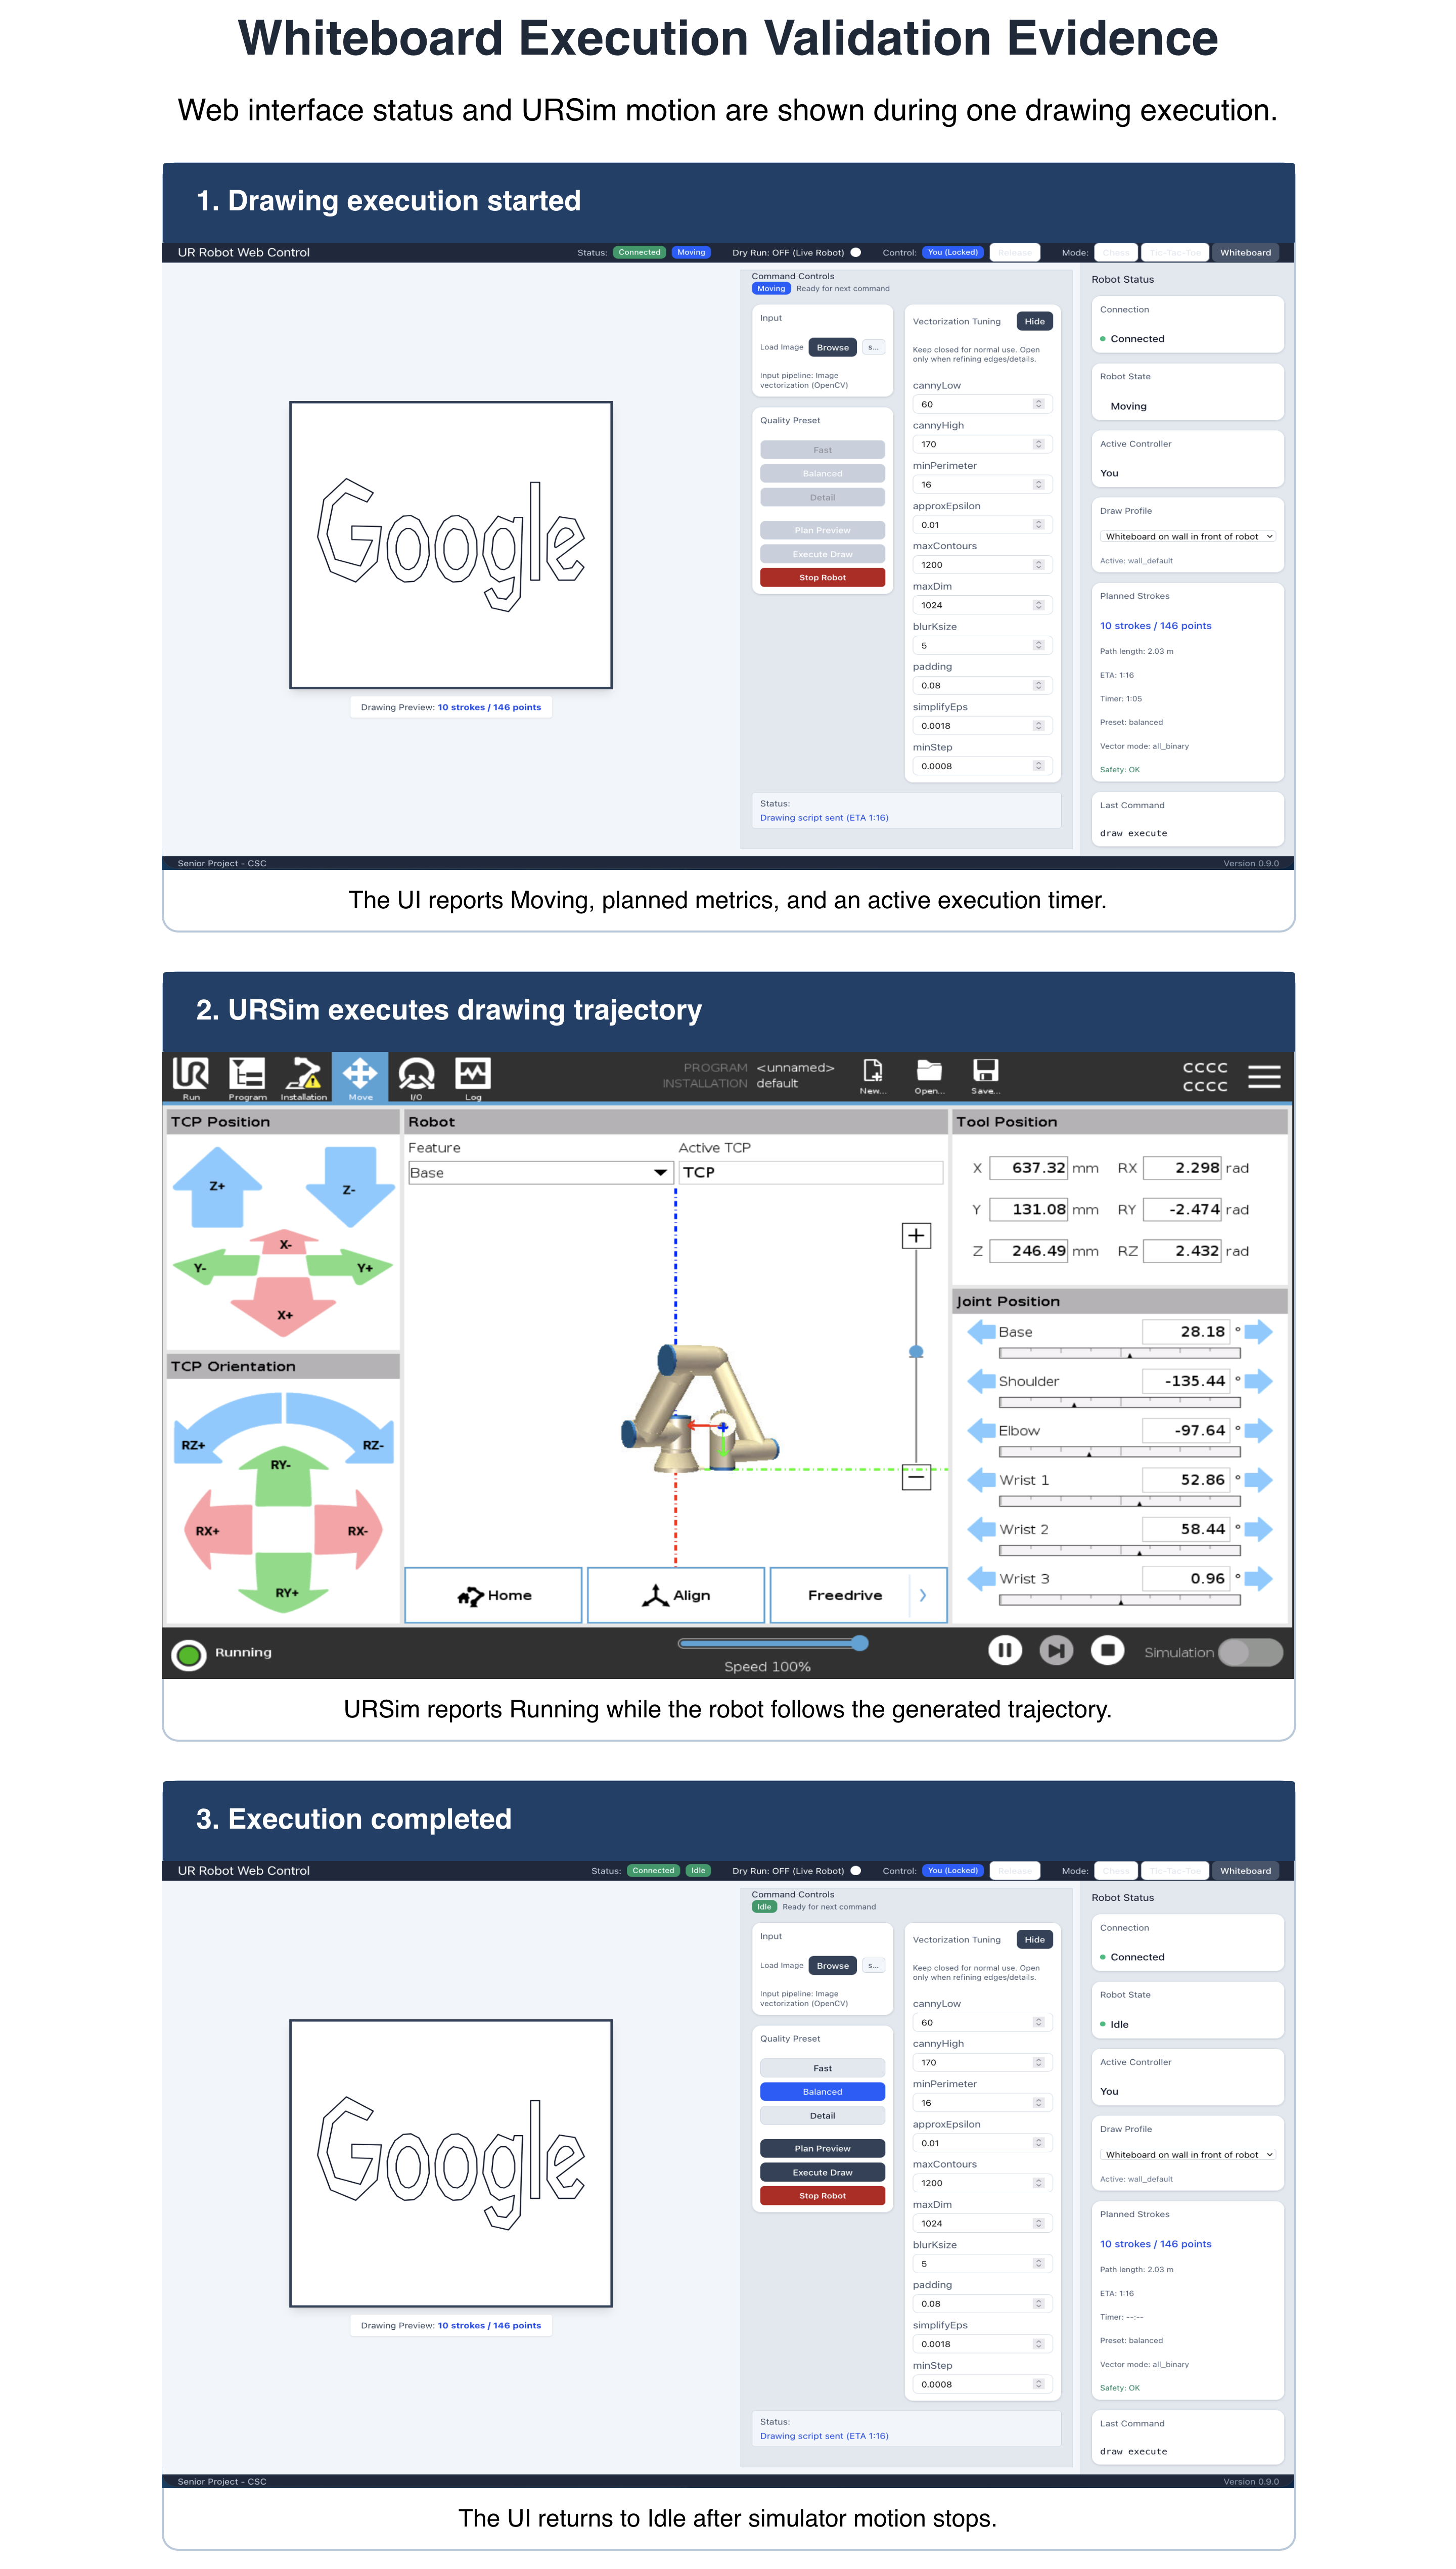
\includegraphics[width=\textwidth,height=0.92\textheight,keepaspectratio]{docs/screenshots/Whiteboard_Execution_Validation.png}
\caption{Whiteboard execution evidence showing UI motion status, URSim execution, and returned idle state.}
\label{fig:whiteboard-execution-validation}
\end{figure}

\subsection{Validation Boundary Summary}
\begin{table}[H]
\centering
\caption{Validation boundary summary.}
\label{tab:functional-validation}
\small
\tablegridon
\begin{tabularx}{\textwidth}{|L{3.0cm}|L{4.8cm}|Y|}
\toprule
Area & Evidence in This Report & Boundary / Limitation \\
\midrule
Board mapping & square/cell selections generated URScript paths and simulator responses & no millimeter-error measurement \tabrowsep
Chess pick / place & same UI/backend flow as board movement & suction transfer not tested \tabrowsep
Tic-tac-toe marking & X/O trajectories generated for selected cells & mark quality and pen contact not tested \tabrowsep
Whiteboard preview/execute & strokes, points, path length, ETA, safety, and script size reported & physical drawing output not measured \tabrowsep
RTDE moving / idle feedback & UI reflected moving/idle transitions with dashboard fallback & latency not quantified \\
\bottomrule
\end{tabularx}
\tablegridoff
\end{table}

\vspace{8.0 em}
\subsection{Metric Coverage Summary}
Table~\ref{tab:metric-coverage} separates collected measurements from metrics that require physical robot testing.

\begin{table}[H]
\centering
\caption{Measured and unmeasured evaluation metrics.}
\label{tab:metric-coverage}
\small
\tablegridon
\begin{tabularx}{\textwidth}{|L{2.8cm}|L{5.6cm}|Y|}
\toprule
Metric Area & Evidence Collected & Not Measured in This Project \\
\midrule
Accuracy & board/cell targets reached intended simulator regions; previews showed stroke fit & placement error, pen offset, suction alignment, camera-verified error \tabrowsep
Timing & whiteboard ETAs: 76~s, 176~s, and 156~s & real execution time, ETA error, network/controller latency \tabrowsep
Repeatability & same inputs and profiles produced same URSim paths & trial variance, hardware drift, long-session repeatability \tabrowsep
Drawing complexity & previews reported strokes, points, script lines, path length & line quality, missed strokes, marker behavior \tabrowsep
Status feedback & moving/idle status observed in UI with dashboard fallback & status latency, false transitions, timing accuracy \\
\bottomrule
\end{tabularx}
\tablegridoff
\end{table}

\subsection{Whiteboard Visual Results}
Figure~\ref{fig:whiteboard-examples} shows the three validation images and the corresponding planned previews generated by the current pipeline. \texttt{sample1.jpg} and \texttt{sample2.png} produced usable previews with the default \texttt{balanced} preset. \texttt{sample3.png} did not: the logo required manual refinement because the default settings over-segmented the shape into many disconnected contour fragments.

\reportfigure[0.99\textwidth]{Whiteboard_Validation_Examples.png}{Input images and planned whiteboard previews.}{fig:whiteboard-examples}

\subsection{Measured Whiteboard Planner Results}
To provide concrete measured outputs, the bundled sample images were tested through the current whiteboard planner using the default \texttt{wall\_default} whiteboard profile. During development, at least 10 logo/image inputs were explored informally. The report shows four whiteboard examples overall, while the repository includes three bundled sample images so the measured results below can be reproduced. The values below were recorded from the preview results shown in the application UI. \texttt{sample1.jpg} and \texttt{sample2.png} used the unmodified \texttt{balanced} preset. \texttt{sample3.png} required light tuning from that preset to obtain a usable preview. ETA values are listed in total seconds even though the UI displays them in \texttt{mm:ss} format.

The table reports continuous pen-down strokes, retained path points, generated URScript motion lines, estimated path length, and planner ETA. Script lines are approximately \texttt{planned points + 2 x planned strokes} because each stroke adds an approach move and a lift move. The ETA values should be interpreted as planner-side estimates for comparing job complexity, not exact completion times. In simulator use, complex or heavily tuned drawings could take longer than the displayed ETA, so real runtime error remains unmeasured.

\begin{table}[H]
\centering
\caption{Measured whiteboard planner results.}
\label{tab:whiteboard-results}
\small
\tablegridon
\begin{tabularx}{\textwidth}{|L{3.0cm}|L{2.0cm}|L{2.0cm}|L{2.0cm}|L{2.1cm}|Y|}
\toprule
Sample Image & Planned Strokes & Planned Points & Script Lines & Path Length (m) & ETA (s) \\
\midrule
\texttt{sample1.jpg} & 10 & 146 & 166 & 2.03 & 76 \\
\texttt{sample2.png} & 19 & 232 & 270 & 4.93 & 176 \\
\texttt{sample3.png} & 4 & 173 & 181 & 4.44 & 156 \\
\bottomrule
\end{tabularx}
\tablegridoff
\end{table}

\subsection{Whiteboard Tuning Result}
Figure~\ref{fig:sample3-tuning} isolates \texttt{sample3.png}, which required manual tuning. With the default \texttt{balanced} preset, the preview produced 88 planned strokes, 269 planned points, and 445 script lines. After reducing \texttt{approxEpsilonFrac} and \texttt{simplifyEpsilon} to their minimum values and setting \texttt{blurKsize=10} in \texttt{all\_binary} mode, the preview was reduced to 4 planned strokes, 173 planned points, and 181 script lines. The tuned preview followed the major outline more cleanly, reducing planned strokes by 84 and script lines by 264 before execution.

\reportfigure[0.99\textwidth]{Whiteboard_Sample3_Tuning.png}{Manual tuning result for \texttt{sample3.png}.}{fig:sample3-tuning}

\subsection{Evaluation Against Criteria}
\begin{table}[H]
\centering
\caption{Evaluation against criteria.}
\label{tab:evaluation}
\small
\tablegridon
\begin{tabularx}{\textwidth}{|L{3.0cm}|L{3.1cm}|Y|}
\toprule
Evaluation Criterion & Outcome & Evidence \\
\midrule
Accuracy & simulator-supported & board and tic-tac-toe targets resolved to intended regions \tabrowsep
Repeatability & qualitative evidence & repeated runs followed the same generated paths for the same profiles \tabrowsep
Status fidelity & observed improvement & RTDE tracked motion state better than fixed timing alone \tabrowsep
Safety compliance & planner checks & draw jobs report stroke count, point count, path length, and script size \tabrowsep
Usability & browser workflow exercised & all three modes operated from one dashboard without manual backend calls \\
\bottomrule
\end{tabularx}
\tablegridoff
\end{table}

\subsection{Results Analysis}
Beyond checking whether each workflow could run, the validation process clarified how the system behaved as an integrated application. The strongest part of the project was the direct mapping path used by the board workflows. Chess movement, chess pick/place sequencing, and tic-tac-toe marking were easier to validate because the user-selected square or cell could be traced through the same sequence each time: UI selection, backend route, calibration profile, generated URScript, URSim response, and UI status update. This made errors easier to isolate because a wrong result usually pointed to either the selected profile, the calibrated anchors, or the generated pose.

Integrating chess, tic-tac-toe, and whiteboard drawing into one architecture showed why the shared layers were useful. Control ownership, calibration profiles, status polling, and URScript dispatch could be reused across all modes, while each task still kept its own planning logic. Chess used discrete square movement and suction state, tic-tac-toe converted a selected cell into bounded mark strokes, and whiteboard mode required image vectorization, tuning, preview metrics, and safety checks. This confirmed the value of the layered, pipeline-based design: common infrastructure reduced duplication, while isolated task modules kept mode-specific complexity from spreading through the rest of the system.

The most important lesson was that the whiteboard workflow is less predictable because it depends on image content before robot planning even begins. During testing, clean high-contrast images produced reasonable previews quickly, while noisy or logo-like inputs required parameter tuning before the planned path looked usable. The most surprising result was that a visually simple output could still have a long planned path: after tuning, \texttt{sample3.png} had only 4 planned strokes but still required 173 points and a 4.44~m path. That changed how the project interpreted validation metrics. Stroke count alone was not enough; point count, path length, script size, visual preview quality, and estimated time all had to be reviewed together before execution.

The measured whiteboard results also showed how quickly complexity changes across inputs. \texttt{sample2.png} produced 19 strokes, 232 points, a 4.93~m planned path, and a 176~s ETA, compared with \texttt{sample1.jpg} at 10 strokes, 146 points, a 2.03~m path, and a 76~s ETA. These values helped make the validation more concrete because they connected preview appearance to measurable planning outputs.

Overall, the system met its main simulation objective: it translated user tasks into executable UR3e behavior through one web interface. The strongest evidence is integrated workflow execution, preview metrics, safety checks, and UI status reporting. The remaining hardware gaps are summarized in Tables~\ref{tab:functional-validation} and~\ref{tab:metric-coverage}.

\section{Limitations and Challenges}
The largest technical challenge was calibration. The system depends on manually defined anchors, so even small setup errors can create visible drift at other target locations. This was especially important for board alignment and whiteboard drawing, where small pose differences are easy to notice.

A second limitation is the simulator-only evaluation. URSim was sufficient for developing the communication path, status logic, and drawing pipeline, but it does not capture physical variation in tool mounting, pen contact, suction behavior, or setup repeatability.

For real hardware, the main safety concerns would be calibration drift, unexpected motion, and tool contact. If the physical board or whiteboard shifts after calibration, a target that appears safe in the UI could map to the wrong physical location. Unexpected motion could also occur if a generated pose is reachable in simulation but awkward for the real arm because of joint limits, tool mounting, or nearby obstacles. Tool contact is especially important for suction and pen-based drawing: too little contact may fail to pick up a piece or mark the board, while too much contact may damage the tool, board surface, or robot setup. A physical deployment should therefore begin with low-speed dry runs above the surface, workspace clearance checks, emergency-stop readiness, and small calibration verification moves before allowing pick/place or pen-down commands.

The whiteboard mode also depends heavily on input image quality. Clean, high-contrast images produce usable previews, while noisy or complex inputs can create weak or overly dense contour plans. ETA is similarly limited: it is useful for comparing jobs, but it does not yet model every factor that affects real execution time.

Finally, the software scope was intentionally constrained. Raster image input is supported, but direct SVG or text workflows were not completed in the final version. This was a deliberate tradeoff to keep the implemented pipeline stable and reviewable rather than expanding into too many partially finished features.

Figure~\ref{fig:limitation} shows a separate input-quality comparison in whiteboard mode. The clean-input preview produced 19 strokes and 2305 points after additional tuning, while the complex-input preview still produced 381 strokes and 4483 points. These counts are not part of the measured sample set in Table~\ref{tab:whiteboard-results}; they are included only to show how image quality and tuning choices can sharply change preview complexity.

\reportfigure[0.85\textwidth]{new_figures/limitation.png}{Whiteboard input-quality limitation.}{fig:limitation}

\section{Future Work}
\begin{itemize}[leftmargin=*]
\item Immediate next step: validate the full pipeline on the physical UR3e by recalibrating anchors, measuring placement and marking repeatability, and comparing real timing against simulator behavior.
\item Near-term software improvements: improve contour fidelity for complex images, optimize stroke ordering, and recalibrate ETA estimates from measured runs.
\item Longer-term extensions: add SVG or text-based drawing workflows, fill or hatching support, and camera-based closed-loop correction for automatic error compensation.
\end{itemize}

\section{Conclusion}
This project developed a web control platform that converts operator inputs into calibrated UR3e behavior. The final system integrates a React and TypeScript frontend, Express route handlers, calibration modules, URScript generation, RTDE-assisted status feedback, and an OpenCV-based drawing pipeline for chess-style movement, tic-tac-toe marking, and whiteboard drawing.

The project demonstrates that a single browser interface can support discrete board movement, bounded marking, and image-driven drawing without exposing the user to raw robot commands. The implemented platform provides end-to-end URSim operation, drawing preview and safety checks, control locking, and live moving/idle feedback. The primary limitation is that physical UR3e validation remains future work. Placement accuracy, suction pickup and release reliability, pen contact behavior, and final drawing quality were not measured on hardware, so the results should be interpreted as URSim-validated software behavior rather than confirmed physical task performance.

\section{Source Code Availability}
The source code for this project is available at:
\url{https://github.com/tkonchok/UR3e_Web_Control.git}

\section{Schedule and Development Milestones}
The project developed iteratively across the two-quarter senior project sequence. The timing below is retrospective and grouped by the major development stages.

\subsection{First Quarter}
\begin{table}[H]
\centering
\caption{First quarter schedule.}
\label{tab:first-quarter}
\small
\tablegridon
\begin{tabularx}{\textwidth}{|L{2.7cm}|L{3.3cm}|Y|}
\toprule
Time Period & Main Focus & Key Deliverables \\
\midrule
Weeks 1--4 & Proposal development and project direction & Defined the initial chess interaction idea, researched tools, and shaped the proposal \tabrowsep
Weeks 5--7 & Scope refinement and feasibility planning & Revised the proposal, simplified scope, and focused on a browser-based UR3e workflow \tabrowsep
Weeks 8--10 & Final proposal preparation & Finalized the proposal direction, confirmed the URSim workflow, and prepared to transition into implementation \\
\bottomrule
\end{tabularx}
\tablegridoff
\end{table}

\subsection{Second Quarter}
\begin{table}[H]
\centering
\caption{Second quarter schedule.}
\label{tab:second-quarter}
\small
\tablegridon
\begin{tabularx}{\textwidth}{|L{2.8cm}|L{3.4cm}|Y|}
\toprule
Time Period & Main Focus & Key Deliverables \\
\midrule
Weeks 1--2 & Proposal finalization and implementation start & Finalized approval and began implementation with simplified scope \tabrowsep
Weeks 3--4 & First board interaction demo and early calibration & Added grid interaction, target selection, robot movement, dry-run mode, control locking, early tic-tac-toe logic, and board anchors \tabrowsep
Weeks 4--5 & Calibration refinement and chess workflow expansion & Improved move-to-square behavior and added chess-piece state tracking for pick/place \tabrowsep
Weeks 5--6 & Robot-side tic-tac-toe marking and UI integration & Added pen-based X/O drawing and unified chess/tic-tac-toe dashboard behavior \tabrowsep
Weeks 7--8 & Structured board interaction expansion & Refined board interactions and integrated board workflows into one interface \tabrowsep
Weeks 8--9 & Chess and whiteboard feature expansion & Connected chess pick/place, image upload, contour extraction, preview, drawing execution, and multi-mode UI \tabrowsep
Week 10 and Finals Week & Refinement, live status, and final report & Added RTDE live status feedback, cleaned the repository, improved documentation, and completed the report \\
\bottomrule
\end{tabularx}
\tablegridoff
\end{table}

\subsection{Milestones}
\begin{itemize}[leftmargin=*]
\item M1: Project idea narrowed to chess-related UR3e interaction through a web interface
\item M2: Proposal finalized with a simplified and realistic scope
\item M3: URSim development workflow and basic command communication established
\item M4: First board interaction demo completed with target-square selection and robot movement
\item M5: Dry-run mode and control locking integrated into the early workflow
\item M6: First version of the three predefined manual anchor points implemented for board calibration
\item M7: Chess piece state integrated into the UI for pick/place tracking
\item M8: Tic-tac-toe robot-side marking implemented with pen-based X/O drawing
\item M9: Whiteboard image upload, contour preview, and drawing execution implemented
\item M10: RTDE live robot status integrated into the UI
\item M11: Final repository cleanup, documentation, and report completed
\end{itemize}

\begin{thebibliography}{18}

\bibitem{goodrich-schultz}
M.~A. Goodrich and A.~C. Schultz.
``Human-Robot Interaction: A Survey.''
\textit{Foundations and Trends in Human-Computer Interaction}, 1(3):203--275, 2007.
\url{https://doi.org/10.1561/1100000005}

\bibitem{hokayem-spong}
P.~F. Hokayem and M.~W. Spong.
``Bilateral Teleoperation: An Historical Survey.''
\textit{Automatica}, 42(12):2035--2057, 2006.
\url{https://doi.org/10.1016/j.automatica.2006.06.027}

\bibitem{web-telepresence}
F.~Melendez-Fernandez, C.~Galindo, and J.~Gonzalez-Jimenez.
``A Web-Based Solution for Robotic Telepresence.''
\textit{International Journal of Advanced Robotic Systems}, 2017.
\url{https://doi.org/10.1177/1729881417743738}

\bibitem{tsai-lenz}
R.~Y. Tsai and R.~K. Lenz.
``A New Technique for Fully Autonomous and Efficient 3D Robotics Hand/Eye Calibration.''
\textit{IEEE Transactions on Robotics and Automation}, 5(3):345--358, 1989.
\url{https://doi.org/10.1109/70.34770}

\bibitem{calibration-review}
I.~Enebuse, M.~Foo, B.~K.~K.~S.~M. Ibrahim, H.~Ahmed, F.~Supmak, and S.~A. Odongo.
``A Comparative Review of Hand-Eye Calibration Techniques for Vision Guided Robots.''
\textit{IEEE Access}, 9:113143--113155, 2021.
\url{https://doi.org/10.1109/ACCESS.2021.3104514}

\bibitem{robotic-sketching}
A.~Mohammed, L.~Wang, and R.~X. Gao.
``Integrated Image Processing and Path Planning for Robotic Sketching.''
\textit{Procedia CIRP}, 12:434--439, 2013.
\url{https://doi.org/10.1016/j.procir.2013.09.035}

\bibitem{urscript-dev}
Universal Robots.
``Develop with URScript.''
\url{https://www.universal-robots.com/developer/urscript/}

\bibitem{urscript-manual}
Universal Robots.
``Script Manual, e-Series.''
\url{https://www.universal-robots.com/download/manuals-e-seriesur-series/script/script-manual-e-series-sw-513/}

\bibitem{rtde-dev}
Universal Robots.
``Real-Time Data Exchange (RTDE).''
\url{https://www.universal-robots.com/developer/communication-protocol/rtde/}

\bibitem{rtde-guide}
Universal Robots.
``Real-Time Data Exchange (RTDE) Guide.''
\url{https://docs.universal-robots.com/tutorials/communication-protocol-tutorials/rtde-guide.html}

\bibitem{dashboard}
Universal Robots.
``Dashboard Server Remote Control Interface e-Series.''
\url{https://www.universal-robots.com/manuals/EN/HTML/SW5_24/Content/prod-dashboard/Dashboard_table.htm}

\bibitem{client-interfaces}
Universal Robots.
``Overview of Client Interfaces.''
\url{https://www.universal-robots.com/articles/ur/interface-communication/overview-of-client-interfaces/}

\bibitem{opencv}
OpenCV.
``OpenCV 4.x Documentation.''
\url{https://docs.opencv.org/4.x/}

\bibitem{numpy}
NumPy Developers.
``NumPy Documentation.''
\url{https://numpy.org/doc/}

\bibitem{express}
Express.js.
``Express Documentation.''
\url{https://expressjs.com/}

\bibitem{react}
React.
``React Documentation.''
\url{https://react.dev/}

\bibitem{vite}
Vite.
``Vite Documentation.''
\url{https://vite.dev/}

\bibitem{node-net}
Node.js.
``Net Module Documentation.''
\url{https://nodejs.org/api/net.html}

\end{thebibliography}

\end{document}
